\documentclass{article}
\usepackage{graphicx} %package to manage images
\usepackage[utf8]{inputenc}
\usepackage[a4paper, total={6in, 8in}]{geometry}
\usepackage{xurl}
\title{Relatório 6 \\ Primeira-análise}
\author{Pedro A. S. O. Neto}
\date{Mar, 2022}

\begin{document}

\maketitle

\section{Total fixações}

Neste relatório eu calculei o tempo que cada participante olhou para cada ROI em dois tipos de trial: 

\begin{itemize}
  \item Trials cujo foco é o Brinquedo Direita
  \item Trials cujo foco é o Brinquedo Esquerda
\end{itemize}

O gráfico da Abacaxi, por exemplo, mostra que, em trials cujo foco é o Brinquedo Direita (D), ela passou mais tempo olhando para o rosto e para o brinquedo da direita. Em trials cujo foco é o Brinquedo Esquerda, ela passou mais tempo olhando para o brinquedo esquerda e para o Rosto, porém também passou algum tempo olhando para Brinquedo Direita.
Safira foi a única criança que tendeu a olhar mais para o Brinquedo Esquerda, quando a ROI era Brinquedo Direita. Mas ela olhou para o Brinquedo Esquerda quando a ROI era Brinquedo Esquerda.

\begin{figure}[t]
\caption{Abacaxi}
\noindent\makebox[\textwidth]{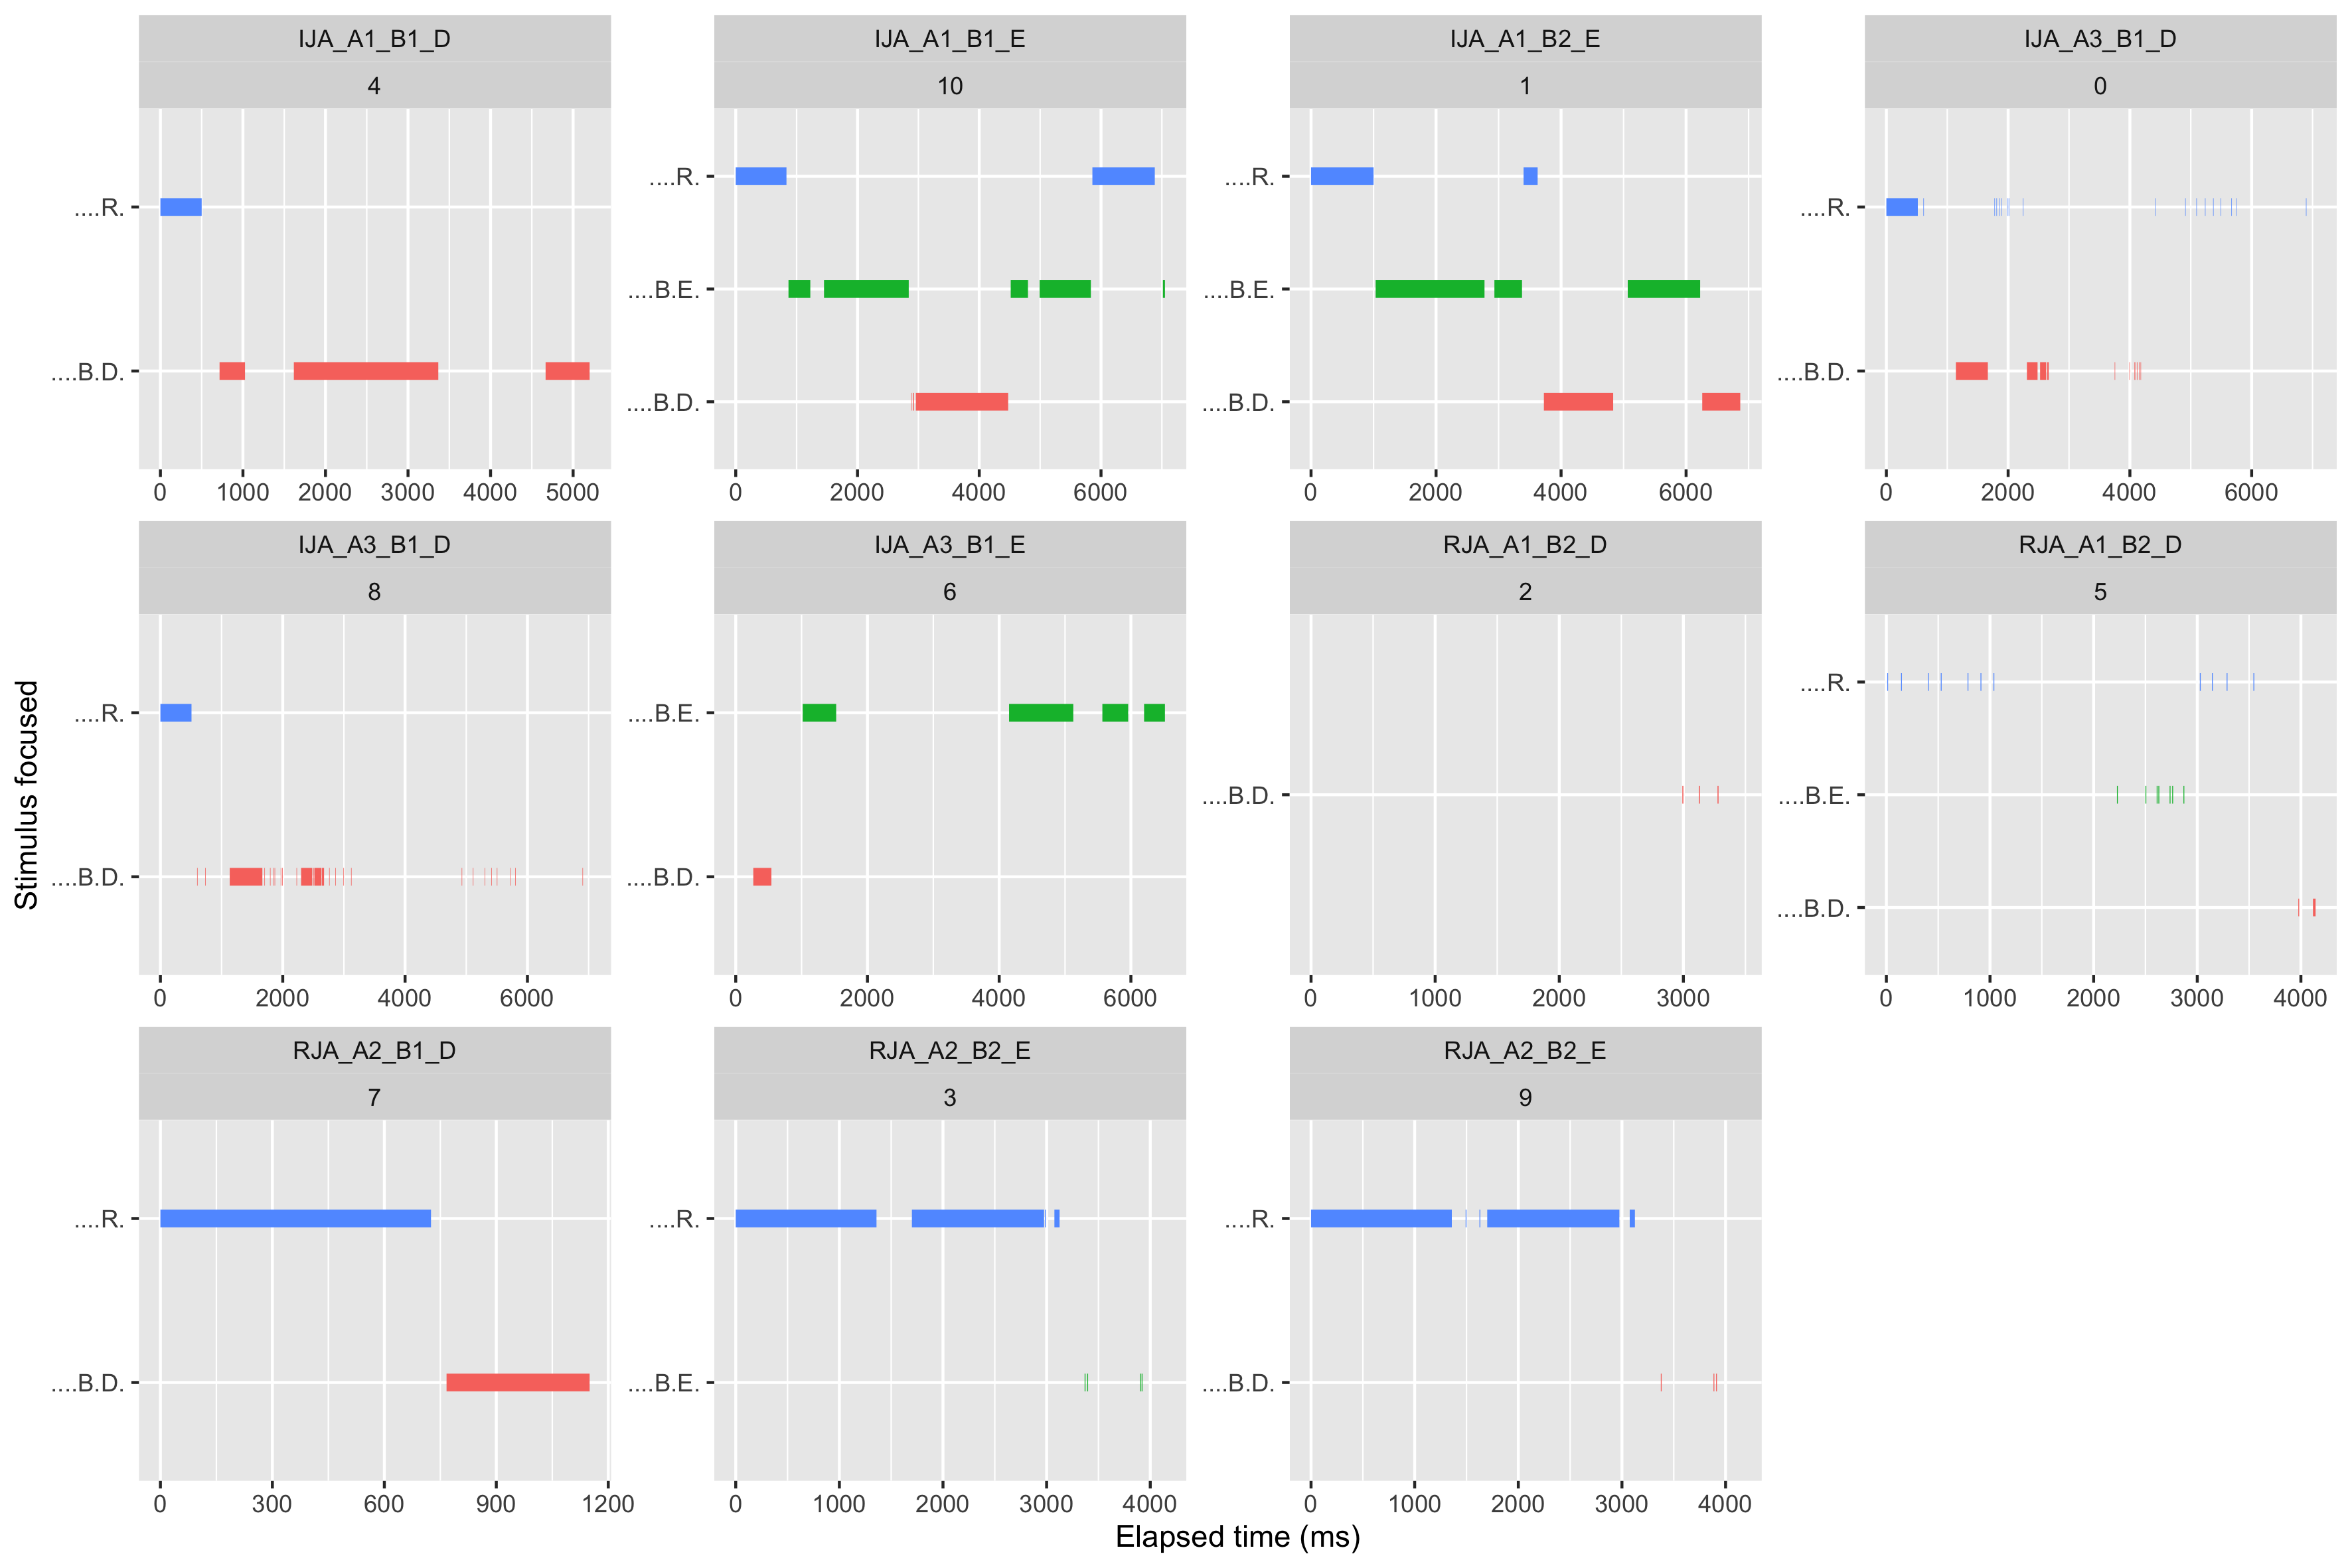
\includegraphics[width=\paperwidth]{"./graph_visu1.png"}}
\centering
\end{figure}

\begin{figure}[t]
\caption{Babacu}
\noindent\makebox[\textwidth]{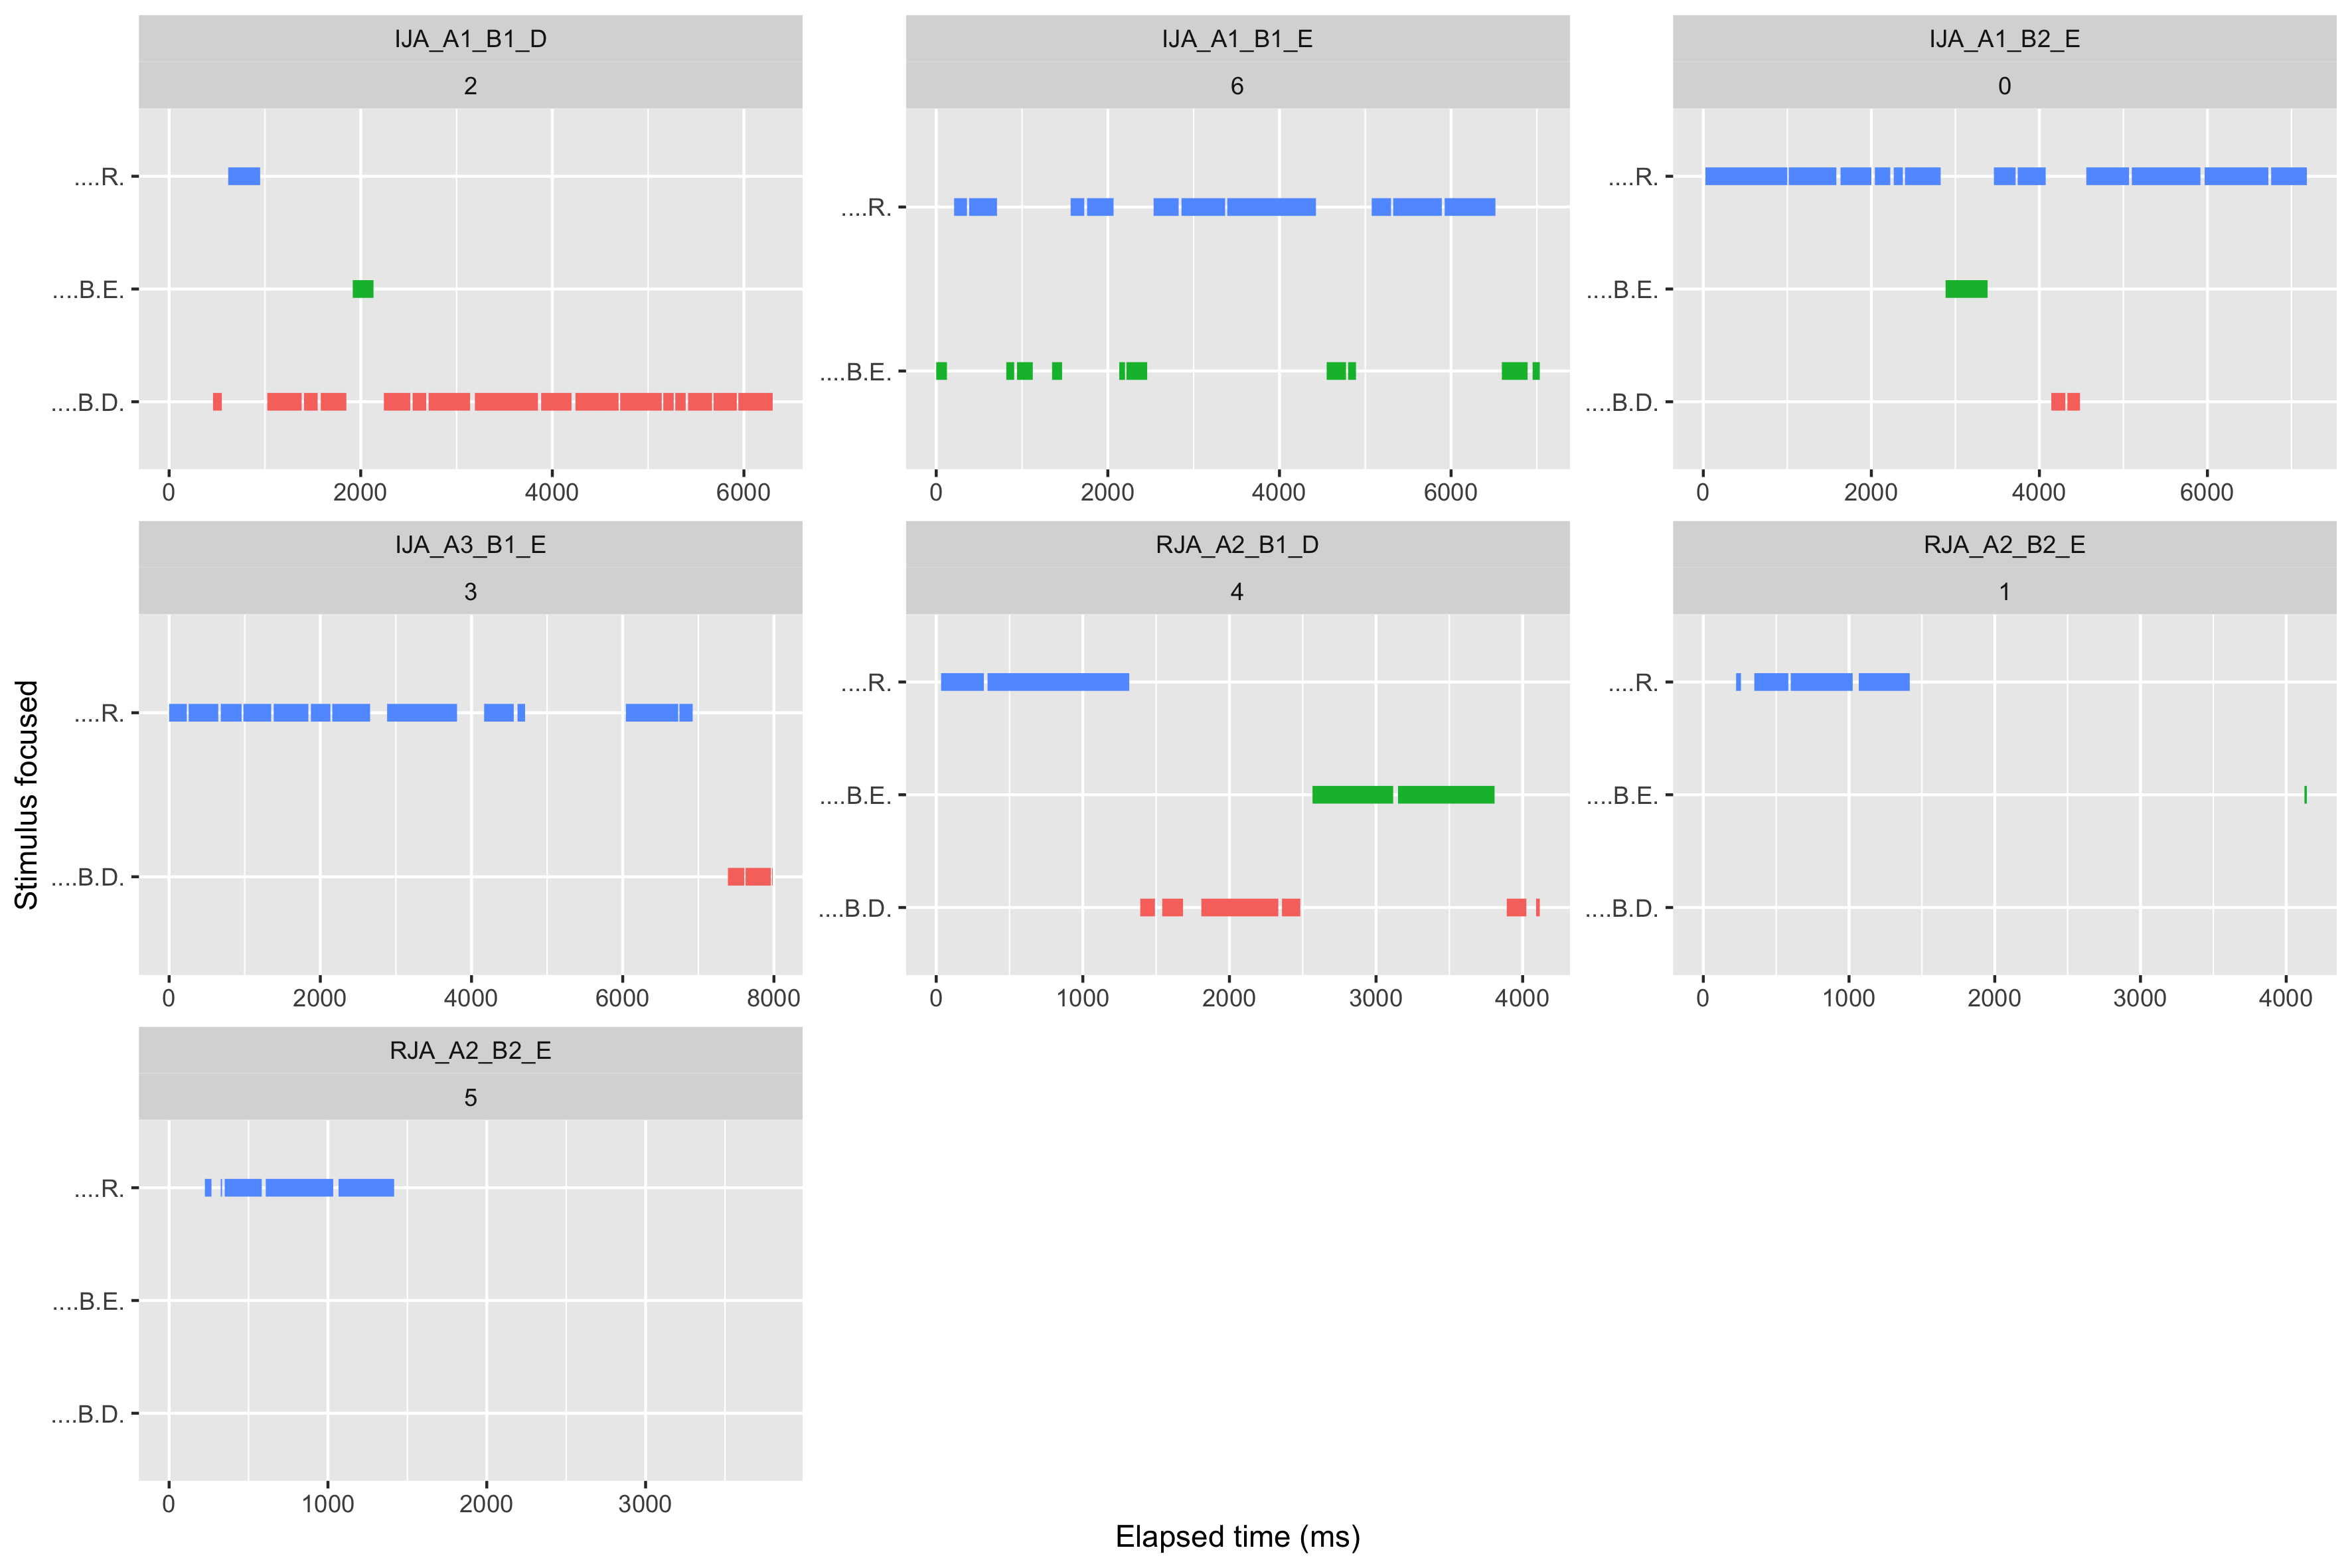
\includegraphics[width=\paperwidth]{"./graph_visu2.png"}}
\centering
\end{figure}

\begin{figure}[t]
\caption{Baru}
\noindent\makebox[\textwidth]{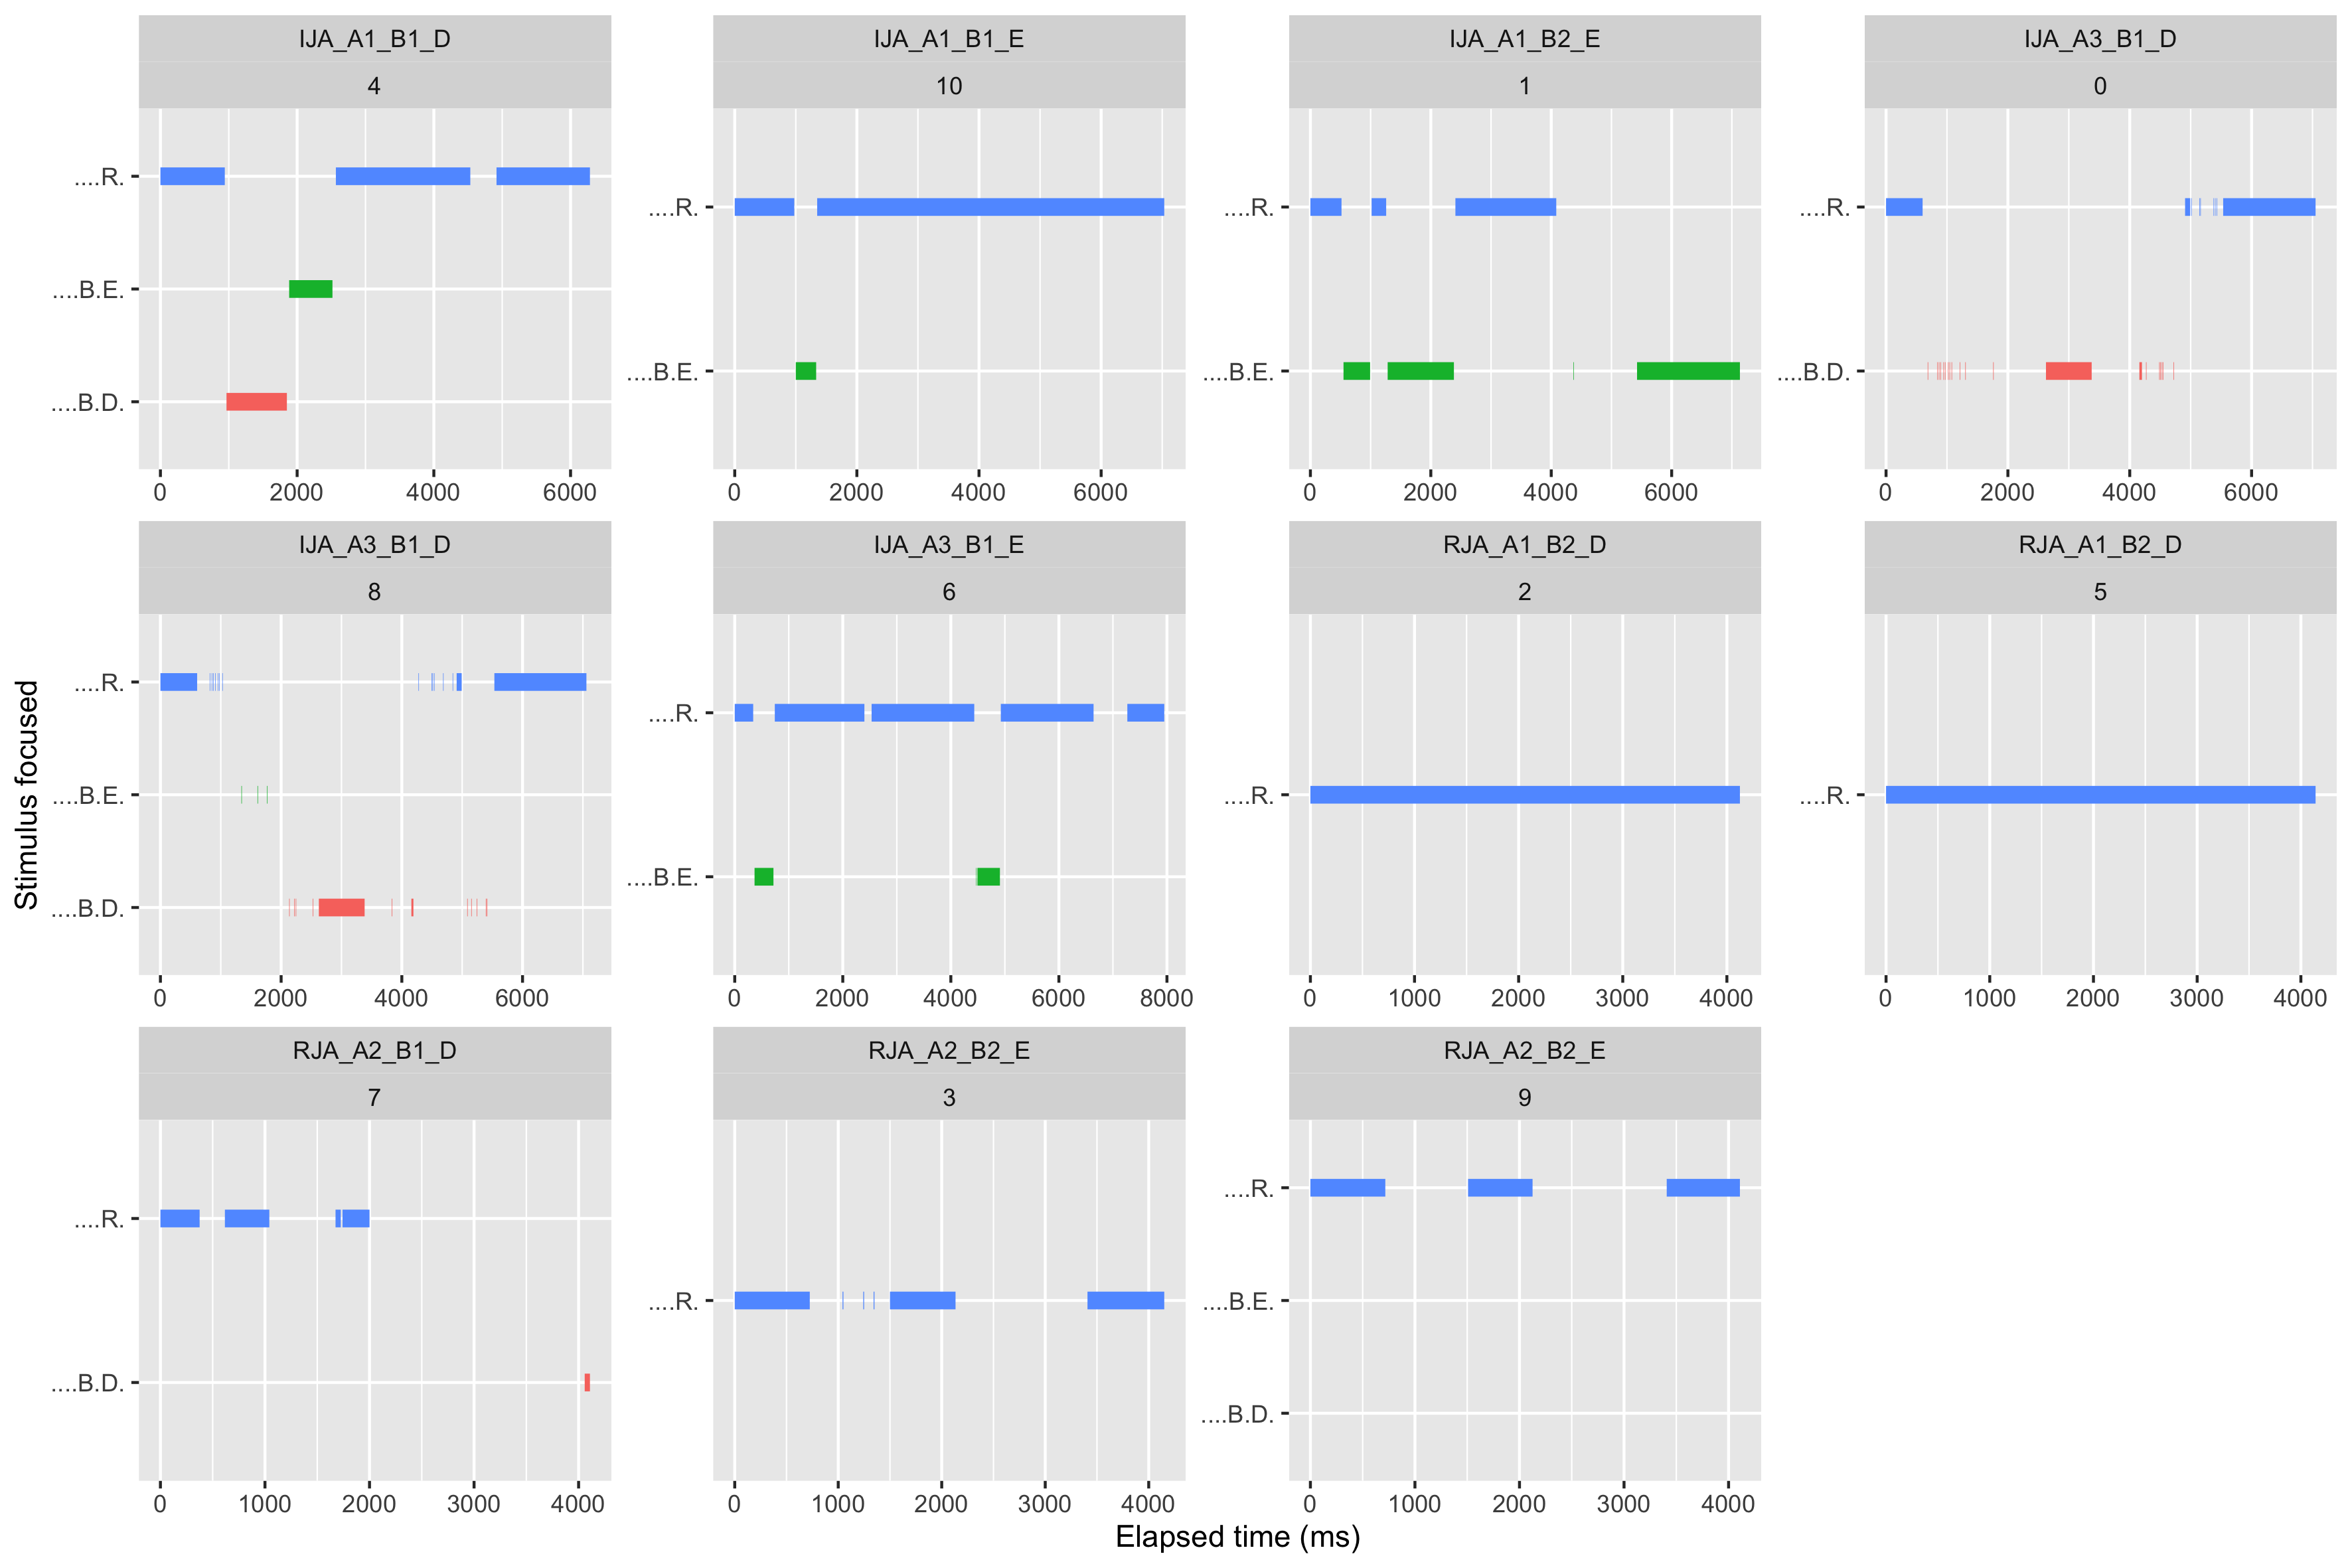
\includegraphics[width=\paperwidth]{"./graph_visu3.png"}}
\centering
\end{figure}

\begin{figure}[t]
\caption{Dovyalis}
\noindent\makebox[\textwidth]{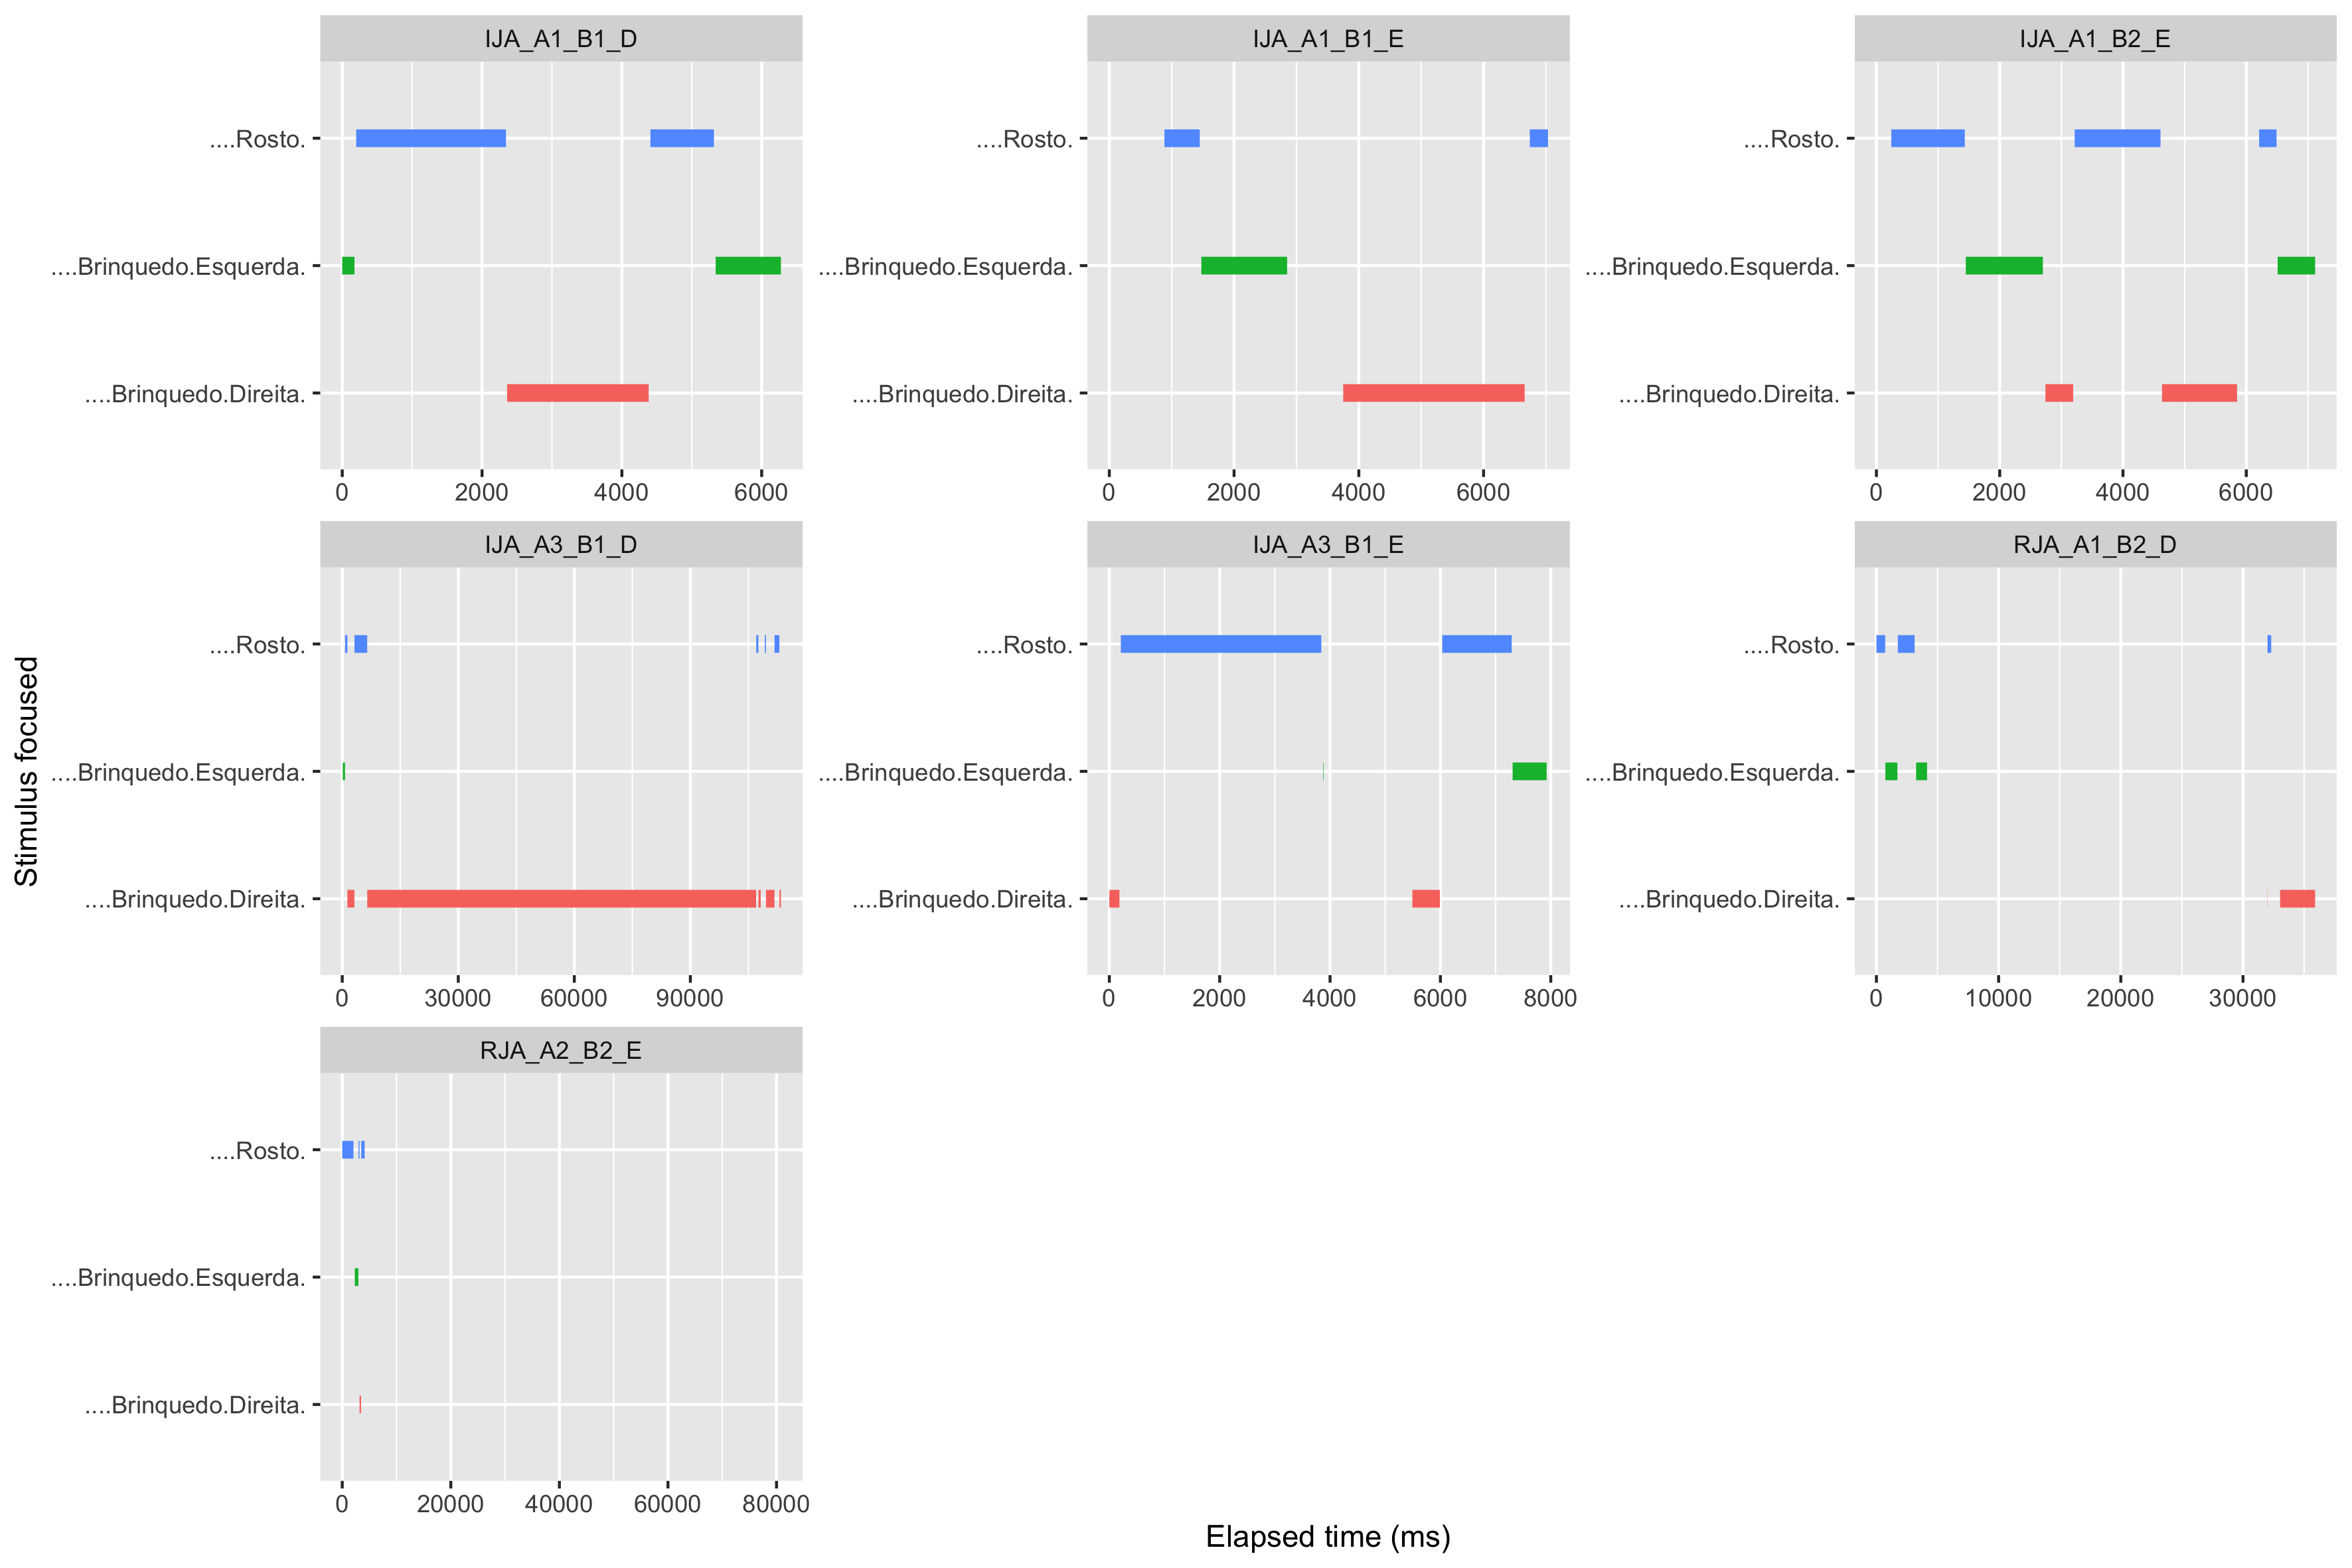
\includegraphics[width=\paperwidth]{"./graph_visu4.png"}}
\centering
\end{figure}

\begin{figure}[t]
\caption{Safira}
\noindent\makebox[\textwidth]{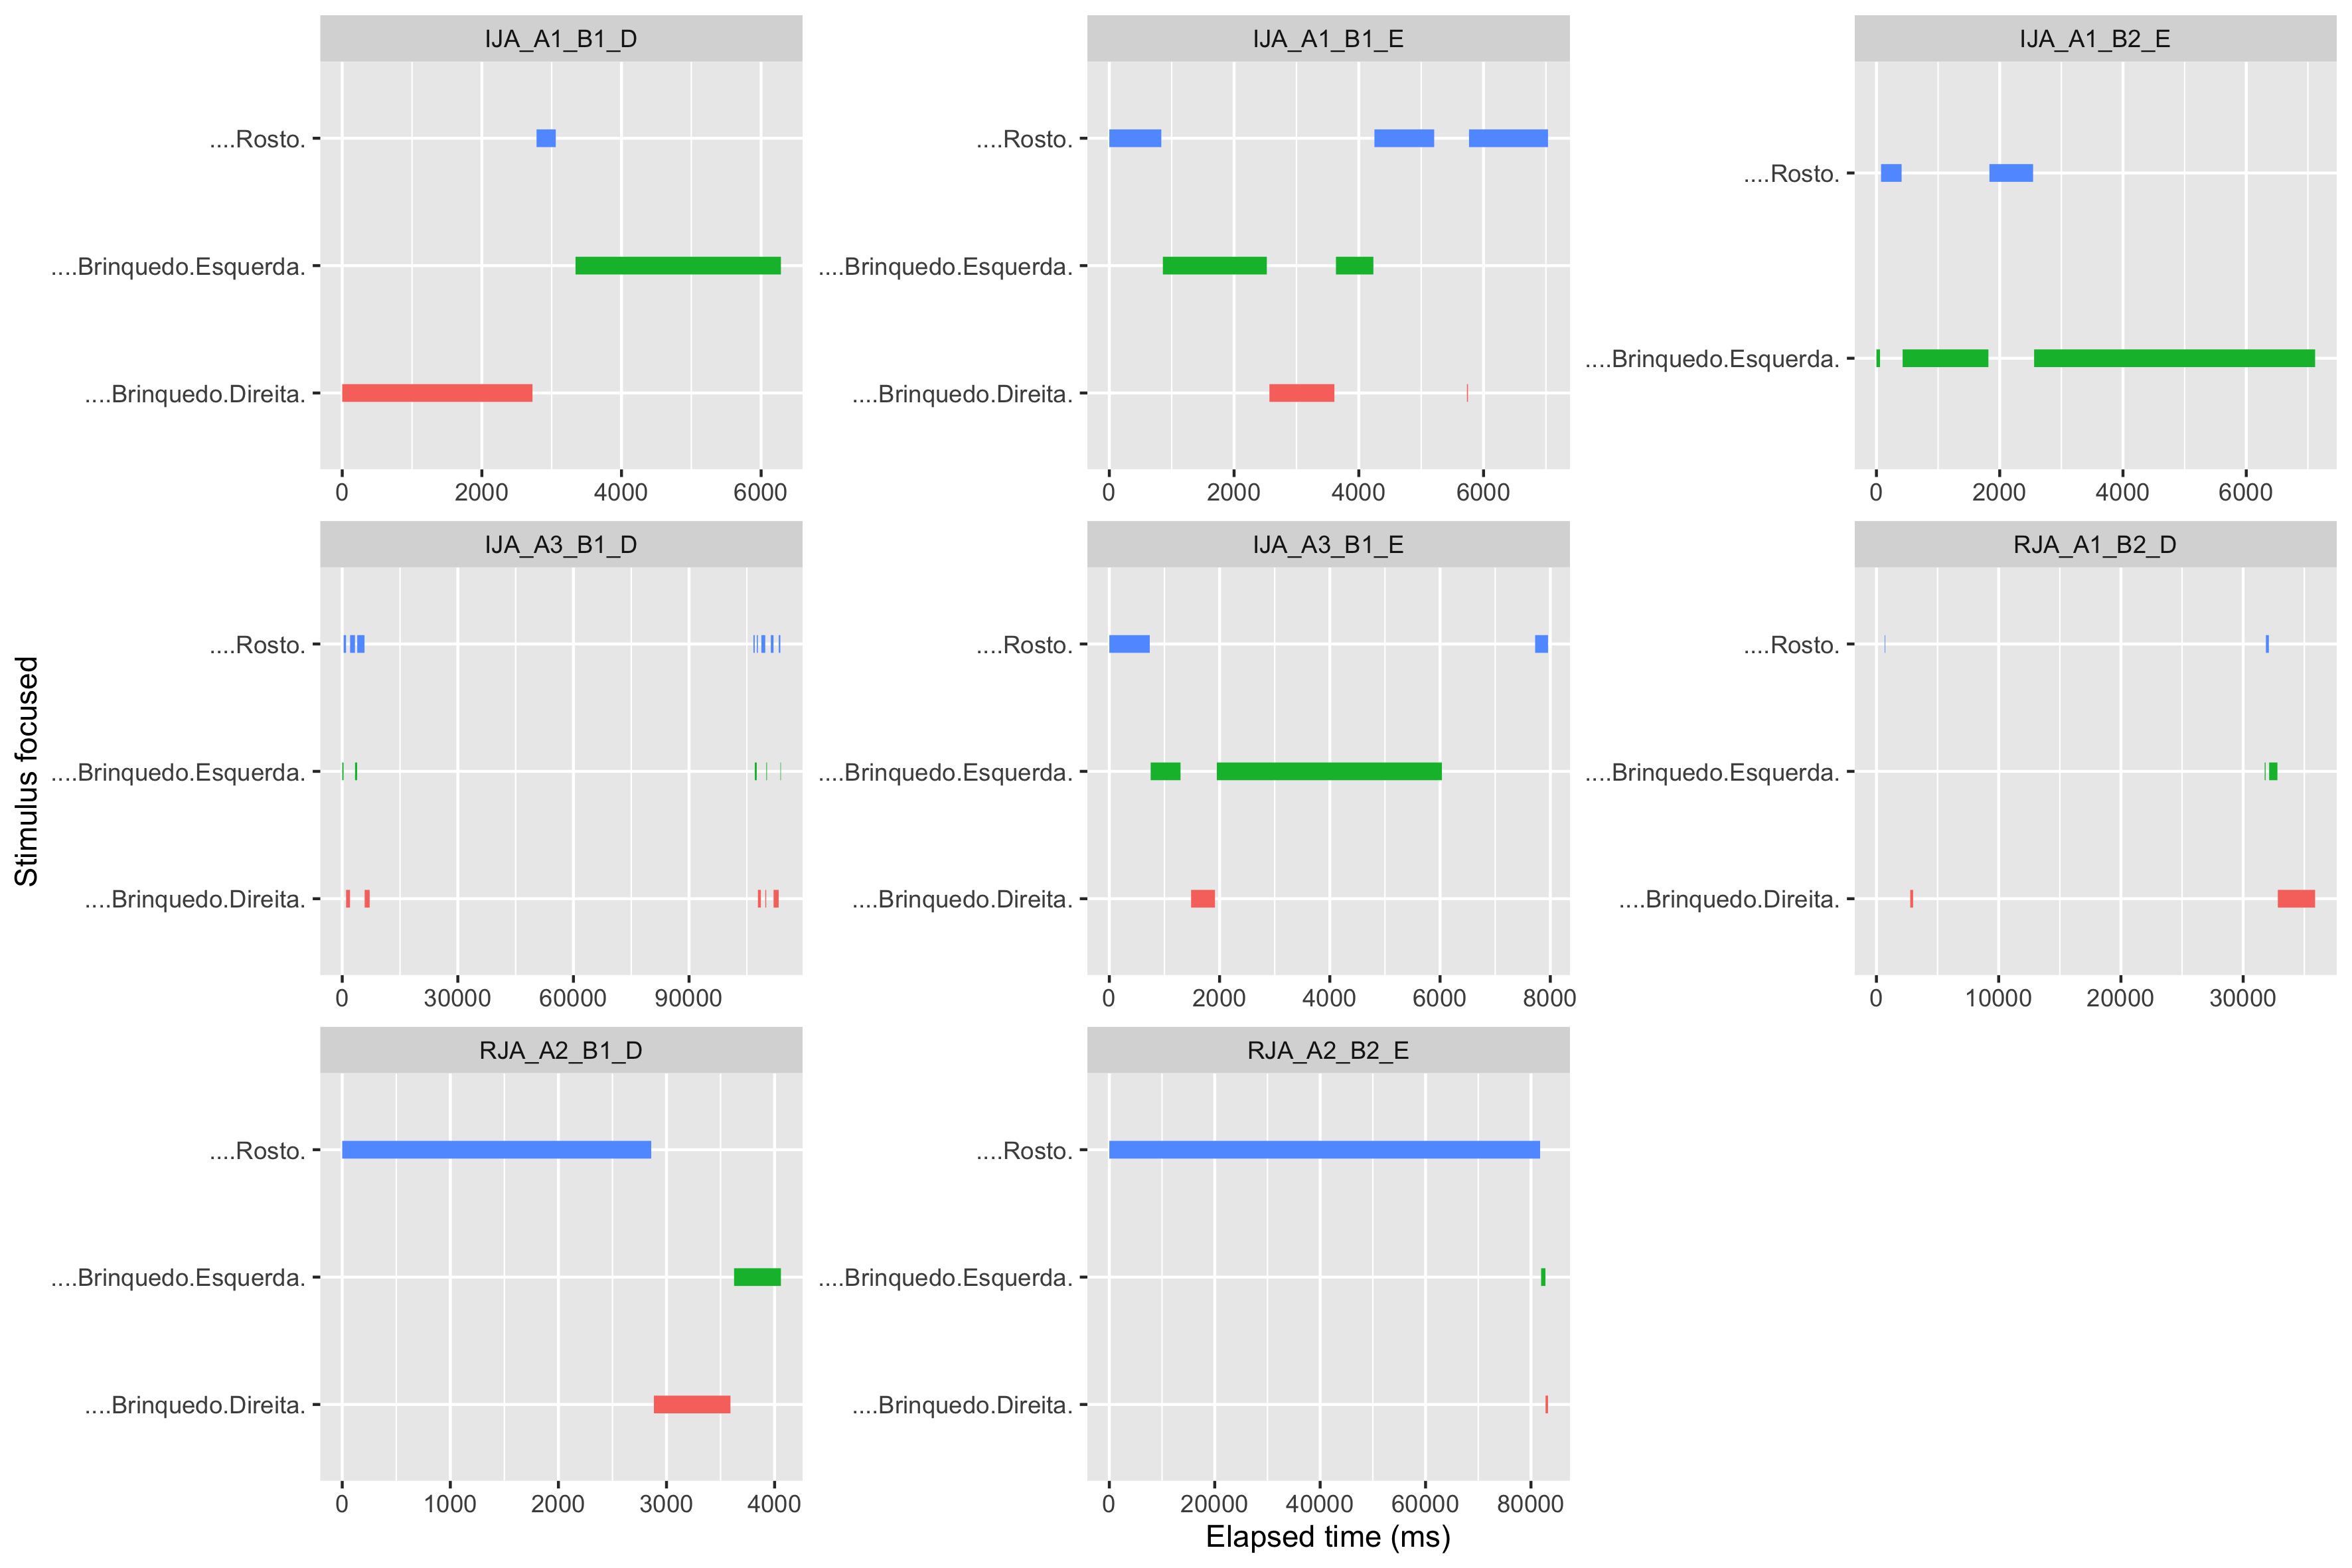
\includegraphics[width=\paperwidth]{"./graph_visu5.png"}}
\centering
\end{figure}

\end{document}


